% !TeX root = ../../master.tex
\section{Probleme und Herausforderungen im Bereich Gouvernance und Observability}

Viele Konzepte, welche für Microservices essenziell sind stellen mit einem strengen Blick auf die Gouvernance und die Observability eine Herausforderung dar. So werden im folgenden Teil einige dieser Konzepte vorgestellt und die damit verbundenen Probleme erläutert. Diese Probleme müssen mithilfe von Tooling oder eventuell sogar Designentscheidungen während der Softwareentwicklung verhindert werden.

\subsection{Design for Failure \autocite{FowlerMicrservices}}
Bei Design for Failure handelt es sich um ein Kernprinzip, welches bereits von \citeauthor{FowlerMicrservices} in seiner Zusammenstellung zu dem Arhcitekturprinzip Microservice in \enquote{\citetitle{FowlerMicrservices}} vorgestellt wurde. Die Idee hinter diesem Prinzip ist, dass Fehler immer, erst Recht im Softwareumfeld unvermeidbar sind. Deshalb müssen 


Design for Failure, aber wie bekomme ich es mit? Wie reagiere ich im Fehlerfall? Was muss getan werden, und wie groß sind die Auswirkungen wenn einer meiner tausend Microservices ausfällt? Diese und viele weitere Fragen müssen sich DevOps und Software-Engerneering Teams oftmals stellen, wenn sie sich in einer dezentralisierten Microservicearchitektur befinden. Es ist oftmals ein tiefes Verständnis des Zusammenspiels der einzelnen Services nötig um heruaszufinden, ob ein Fehler von eigenen Service kommt, oder ob es aufgrund eines Fehlers in einem anderen Service kommt. Das ultimative Ziel ist es dabei herauszufinden was das Problem ist und dieses auch schnellstmöglich zu beheben, sodass für den Endnutzer keine Merkbaren folgen auftreten. Microservices folgen dm Prinzip "Design for Failure", sodass eine Recovery möglich ist und ein operatives Business aufrecht erhalten werden kann. Trotz dieser hervorragenden Prämisse reicht ein \enquote{Design for Failure} alleine nicht aus. \enquote{Ein System ist nur so schlau wie das schwächste seiner Bestandteile}. Microservices mit dem Ziel kleiner dezentralisierter Services, welche einen spezialisiert sind auf eine bestimmte aufgabe innerhalb eines BusinessProzesses haben ironischerweise eine ihrer größten Schwäche in der Kommunikation miteinander. Es müssen Standards etabliert werden, sodass ServiceOwner einen wartbaren und funktionsfähigen Service entwickeln können. Es muss einen Software-Engeneer an einer Stelle ein Fehler unterlaufen und aufgrund der starken Kohäsion und Abhängigkeit der einzelnen Services unterneinander kann eine Reihe wichtiger Businessfunktionen davon betroffen sein. Im Beipsiel von Amazon führte ein Fehler in einem Service zu einer 20 Minütigen Downtime der Verkaufswebsite, was einem monetären Verlust von ca. 3.5 Mio Euro gleichkommt.

Kein Problem - \enquote{Design for Failure}. Ein Service fällt aus und ist darauf ausgelegt sich selbst wieder zu reaktivieren. Alle anderen Services können einen ausfall händeln. Soweit die Theorie. In der Praxis ist das leider nur allzuoft nicht der Fall. Innerhalb der Microservice-Gouvernance steht der Aspekt der dezentralisierten Entscheidungsfindung im Vordergrund. Das bedeutet, dass jedes Team das fachliche und unternehmerische Know-How zugesprochen wird das beste Tool und die beste Technologie für die von ihnen zu lösende Aufgabe zu wählen. Fängt ein Architekt nun an diese Aufgabe zu lösen, so benötigt er oftmals Informationen aus anderen Microservices, um seine Aufgabe zu erfüllen. 


\begin{center}
	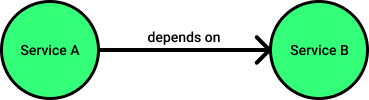
\includegraphics[width=0.55\linewidth]{img/service_dependency.png}
\end{center}

Es entsteht also eine Abhängigkeit zwischen zwei Microservices. Ebendieser angefragte Microservice benötigt aber wiederum einen anderen Service, um die angeforderte Information generieren zu können. Es entsteht also schon eine Kette von Abhängigkeiten. Was passiert, wenn ein Glied dieser Kette einen Fehler wirft? 

\Large Hier kommt ein Bild von einem Fehler in einer Microsericekette

\normalsize

Kein Problem - \enquote{Design for Failure}. Ein Architekt muss in der Planung seines Services die Möglichkeit haben, das Risiko und die Auswirkungen einen Ausfalls sowohl seines eigenen Services, als auch seiner Abhängigkeiten einschätzen zu können. Diese Einschätzung sollte auf Daten basieren, welche sowohl Information bisheriger Ausfälle und deren Ursachen enthalten als auch Ausblicke geben können auf den aktuellen Stand und eventuelle zukünftige Ausfälle.

Wie bereits Eingangs erwähnt ist bei der Betrachtung dieses Prinzips die Brille der Gouvernance und Observability aufgesetzt. Es ist ein wichtiger Bestandteil die Services innerhalb einer Unternehmensarchitektur so aufzubauen, dass diese trotz eins Fehlers ordnungsgemäß weiterlaufen und die Fähigkeit zur Recovery besitzen. Dieses Prinzip ist sogar dafür Veranwtortlich, dass Microservicepioniere wie Netflix innerhalb der Observability eine eigene, vierte Säule zu etablieren. Dabei handelt es sich um das sogenannte Chaos-Testing. Um dies kurz zu erläutern: Dabei handelt es sich um einen eigenen \enquote{Service}, welcher auf Basis von Chaos-Experimenten produktive Services ausschaltet und so die Recovery ebendieses Services und auch der davon abhängigen Services überprüfen kann. Dies bringt viele Vorteile mit sich und sorgt auch dafür, dass Services gut entwickelt sind. Diese Idee, wie das bewusste Einführen von Fehlern die generelle Qualität von Services verbessern kann, wird näher in \citetitle{AntifragileOrganization}\autocite{AntifragileOrganization} beschrieben.

\begin{itemize}
	\item Abgrenzung von Microservices gegenüber API's \\
	Wenn von Microservice Gouvernance und Observability geredet wird, ist oftmals die unterleigende Architektur mit Fokus auf VM-Daten usw gemeint. Wird von APIS gesprchen hat es oftmals mit business logik undso zutun
\end{itemize}
\begin{itemize}
	\item Welcher bereich soll observiert werden?
	\begin{itemize}
		\item Soll es um die hardware Daten (Memory, CPU, klassische cloud metriken) gehen oder um
		\item Softwareinformationen bzgl. software logging und tracing
	\end{itemize}
\end{itemize}
